\appendix
\chapter{Glossary}

These terms are used interchangeably throughout the dissertation, to not tire the reader by using the same term repeatedly.

\begin{itemize}
    \item Timetable = Schedule = Itinerary
    \item Duty = Shift 
    \item Break = Meal-Relief
    \item HGV = Heavy Goods Vehicles = 7.5 tonne lorries
    \item HGV Driver = Employee
    \item Model = Formulation 
\end{itemize}

\vspace{\baselineskip}
\noindent
Unless stated otherwise, all \textbf{time} values are presented in (HH:mm) format. 
 
 %%%%%%%%%%%%%%%%%%%%%%%%%%%%%%%%%%%%%%%%%%%%%%%%%%%%%%%% CHAPTER %%%%%%%%%%%%%%%%%%%%%%%%%%%%%%%%%%%%%%%%%%%%%%%%%%%%%%%%%%%%%%%%%%%%%

\chapter{Second Appendix}
\label{chapter: second appendix}
Tables showing the characteristics of the Historical Schedule. Number of input components, average, minimum, maximum duty lengths in (HH:mm), and overall time scheduled.

\todo{put this as a clarifying note}
%%%%%%%%%%%%%%%%%%%%%%%%%%%%%%%%%%%%%%%%%%%%%%%%%%%%%%%% Section %%%%%%%%%%%%%%%%%%%%%%%%%%%%%%%%%%%%%%%%%%%%%%%%%%%%%%%%%%%%%%%%%%%%%%%%%

\section{Dataset Findings}
In this section of the appendix, we mention some interesting facts that were observed during the study of the historical schedules that we not deemed important enough to display in the main part of the port. However, we believe that they are useful for reference purposes which is why we outline them below. 

%%%%%%%%%%%%%%%%%%%%%%%%%%%%%%%%%%%%%%%%%%%%%%%%%%%%%%%% sub-Section %%%%%%%%%%%%%%%%%%%%%%%%%%%%%%%%%%%%%%%%%%%%%%%%%%%%%%%%%%%%%%%%%%%%%%%%%

\subsection{Attributes Featured in the Dataset}
\label{subsection: Eliminated Attributes}
In the following section we outline a detailed list of the attributes observed in the dataset as well as a description of the information they provide. As mentioned in Section \ref{section: Data Cleaning} of Chapter \ref{chapter: Problem Definition} we preserve information from only a handful of them and the rest are taken into account for the purposes of this project.

%%%%%%%%%%%%%%%%%%%%%%%%%%%%%%%%%%%%%%%%%%%%%%%%%%%%%%%%%%%%%%%%%%%%%% Table %%%%%%%%%%%%%%%%%%%%%%%%%%%%%%%%%%%%%%%%%%%%%%%


%Table containing the types of activities
\begin{table}[ht]
\small
    \centering 
    \begin{tabular}{|l|p{8.3cm}|}
        \hline
       \multicolumn{1}{|c|}{ \textbf{Activity}} & \multicolumn{1}{|c|}{ \textbf{Description}} \\
        \hline
        \texttt{Operator}  & Indicates the ID of the operator that structured each duty. \\
        \hline
        \texttt{Sort\_Order}  & Attaches a unique ID to every activity. \\
        \hline
        \multirow{2}*{\texttt{Duty\_ID}}  & Provides each duty with a unique code for identification purposes. \\ 
        \hline
        \multirow{2}*{\texttt{Date\_Amended} } & Mentions the date that the particular duty was last modified.   \\ 
        \hline
       \texttt{Commencement Time}  & Start time of each activity. \\     
        \hline
       \texttt{Ending Time}  & End time of each activity. \\
        \hline
        \texttt{Element Type}  & Mentions the type of each activity. \\     
        \hline
        \texttt{Element Time}  & Contains the duration of each activity. \\    
        \hline
        \texttt{Due to Convey}   & Mentions the purpose of each \texttt{travel} activity. \\ 
        \hline
        \multirow{2}*{\texttt{Vehicle Type}}  & Mentions the type of HGV vehicle utilised for each travel leg. \\ 
        \hline
        \texttt{From\_Site}  & Contains the start location at which each activity occurs. \\ 
        \hline
        \multirow{2}*{\texttt{To\_Site}}  & Contains the end location at which each activity is completed. \\ 
        \hline
        \multirow{2}*{\texttt{Driver\_Grade}}  & Mentions the qualification of the driver undertaking each activity. \\ 
        \hline
        \multirow{2}*{\texttt{Leg\_Mileage}}  & Contains information about the distance (in miles) of each travel leg. \\ 
        \hline
    \end{tabular}%
    \medbreak
    \caption{List of the types of attributes featured in the dataset.}
    \label{table:Attribute List}
\end{table}

%%%%%%%%%%%%%%%%%%%%%%%%%%%%%%%%%%%%%%%%%%%%%%%%%%%%%%%% sub-Section %%%%%%%%%%%%%%%%%%%%%%%%%%%%%%%%%%%%%%%%%%%%%%%%%%%%%%%%%%%%%%%%%%%%%%%%%

\subsection{Activities Featured in the Dataset}
\label{section: Appendix Activities Feaure in the Dataset}
The activities seen in Table \ref{table:Activity List} were those that were observed in the original form of the dataset as was provided to us by Royal Mail. Upon the implementation of the Data Cleaning procedures as seen in Section \ref{section: Data Cleaning} of Chapter \ref{chapter: Problem Definition}, the list of activities was transformed to its \textbf{Finalised Dataset} form as seen in Table \ref{table:Final Activity List} of Section \ref{section: Data Cleaning}.

%%%%%%%%%%%%%%%%%%%%%%%%%%%%%%%%%%%%%%%%%%%%%%%%%%%%%%%%%%%%%%%%%%%%%% Table %%%%%%%%%%%%%%%%%%%%%%%%%%%%%%%%%%%%%%%%%%%%%%%


%Table containing the types of activities
\begin{table}[ht]
\small
    \centering 
    \begin{tabular}{|l|p{8.3cm}|}
        \hline
       \multicolumn{1}{|c|}{ \textbf{Activity}} & \multicolumn{1}{|c|}{ \textbf{Description}} \\
        \hline
        \texttt{Start}  & Indicates the \textit{beginning} of a duty. \\
        \hline
        \texttt{End}  & Indicates the \textit{end} of a duty. \\
        \hline
        \texttt{Travel}  & The \textit{travel leg} from one location to the next. \\ 
        \hline
        \texttt{Load}  & The \textit{loading} of mail units before leaving a location.   \\ 
        \hline
        \multirow{2}*{\texttt{Unload}}  & The \textit{offloading} of mail units after arriving at a designated location.   \\ 
        \hline
        \multirow{2}*{\texttt{Meal-Relief}}  & The \textit{meal allowance} break to meet EU \textit{driving time} regulations. \\ 
        \hline
       \texttt{Distribution}  & Non-essential administrative tasks. \\     
        \hline
        \texttt{Processing}  & Non-essential administrative tasks. \\     
        \hline
        \texttt{Park Vehicle}   & \textit{Parking} of HGV at end of duty. \\ 
        \hline
        \texttt{Check}  & Scheduled \textit{servicing} of HGV. \\ 
        \hline
        \texttt{Clean}  & Scheduled \textit{cleaning} of HGV. \\ 
        \hline
    \end{tabular}%
    \medbreak
    \caption{List of the types of activities, as featured in the dataset.}
    \label{table:Activity List}
\end{table}

%%%%%%%%%%%%%%%%%%%%%%%%%%%%%%%%%%%%%%%%%%%%%%%%%%%%%%%% sub-Section %%%%%%%%%%%%%%%%%%%%%%%%%%%%%%%%%%%%%%%%%%%%%%%%%%%%%%%%%%%%%%%%%%%%%%%%%

\subsection{Starting Times of Duties}
\label{subsection: Appendix Starting times}
As was mentioned in the Data Exploration section \ref{section: Data Exploration}, the duties of each driver tend to start in \textit{clusters}, internally referred to as \textbf{waves}. This is clearly observed in Figure \ref{fig:starting time} where we have plotted the \textit{starting times} of duties, with the duties sorted in an increasing order. 

%%%%%%%%%%%%%%%%%%%%%%%%%%%%%%%%%%%%%%%%%%%%%%%%%%%%%%%% Figure %%%%%%%%%%%%%%%%%%%%%%%%%%%%%%%%%%%%%%%%%%%%%%%%%%%%%%%%%%%%%%%%%%%%%%%%%


\begin{figure}[ht]
\begin{center}
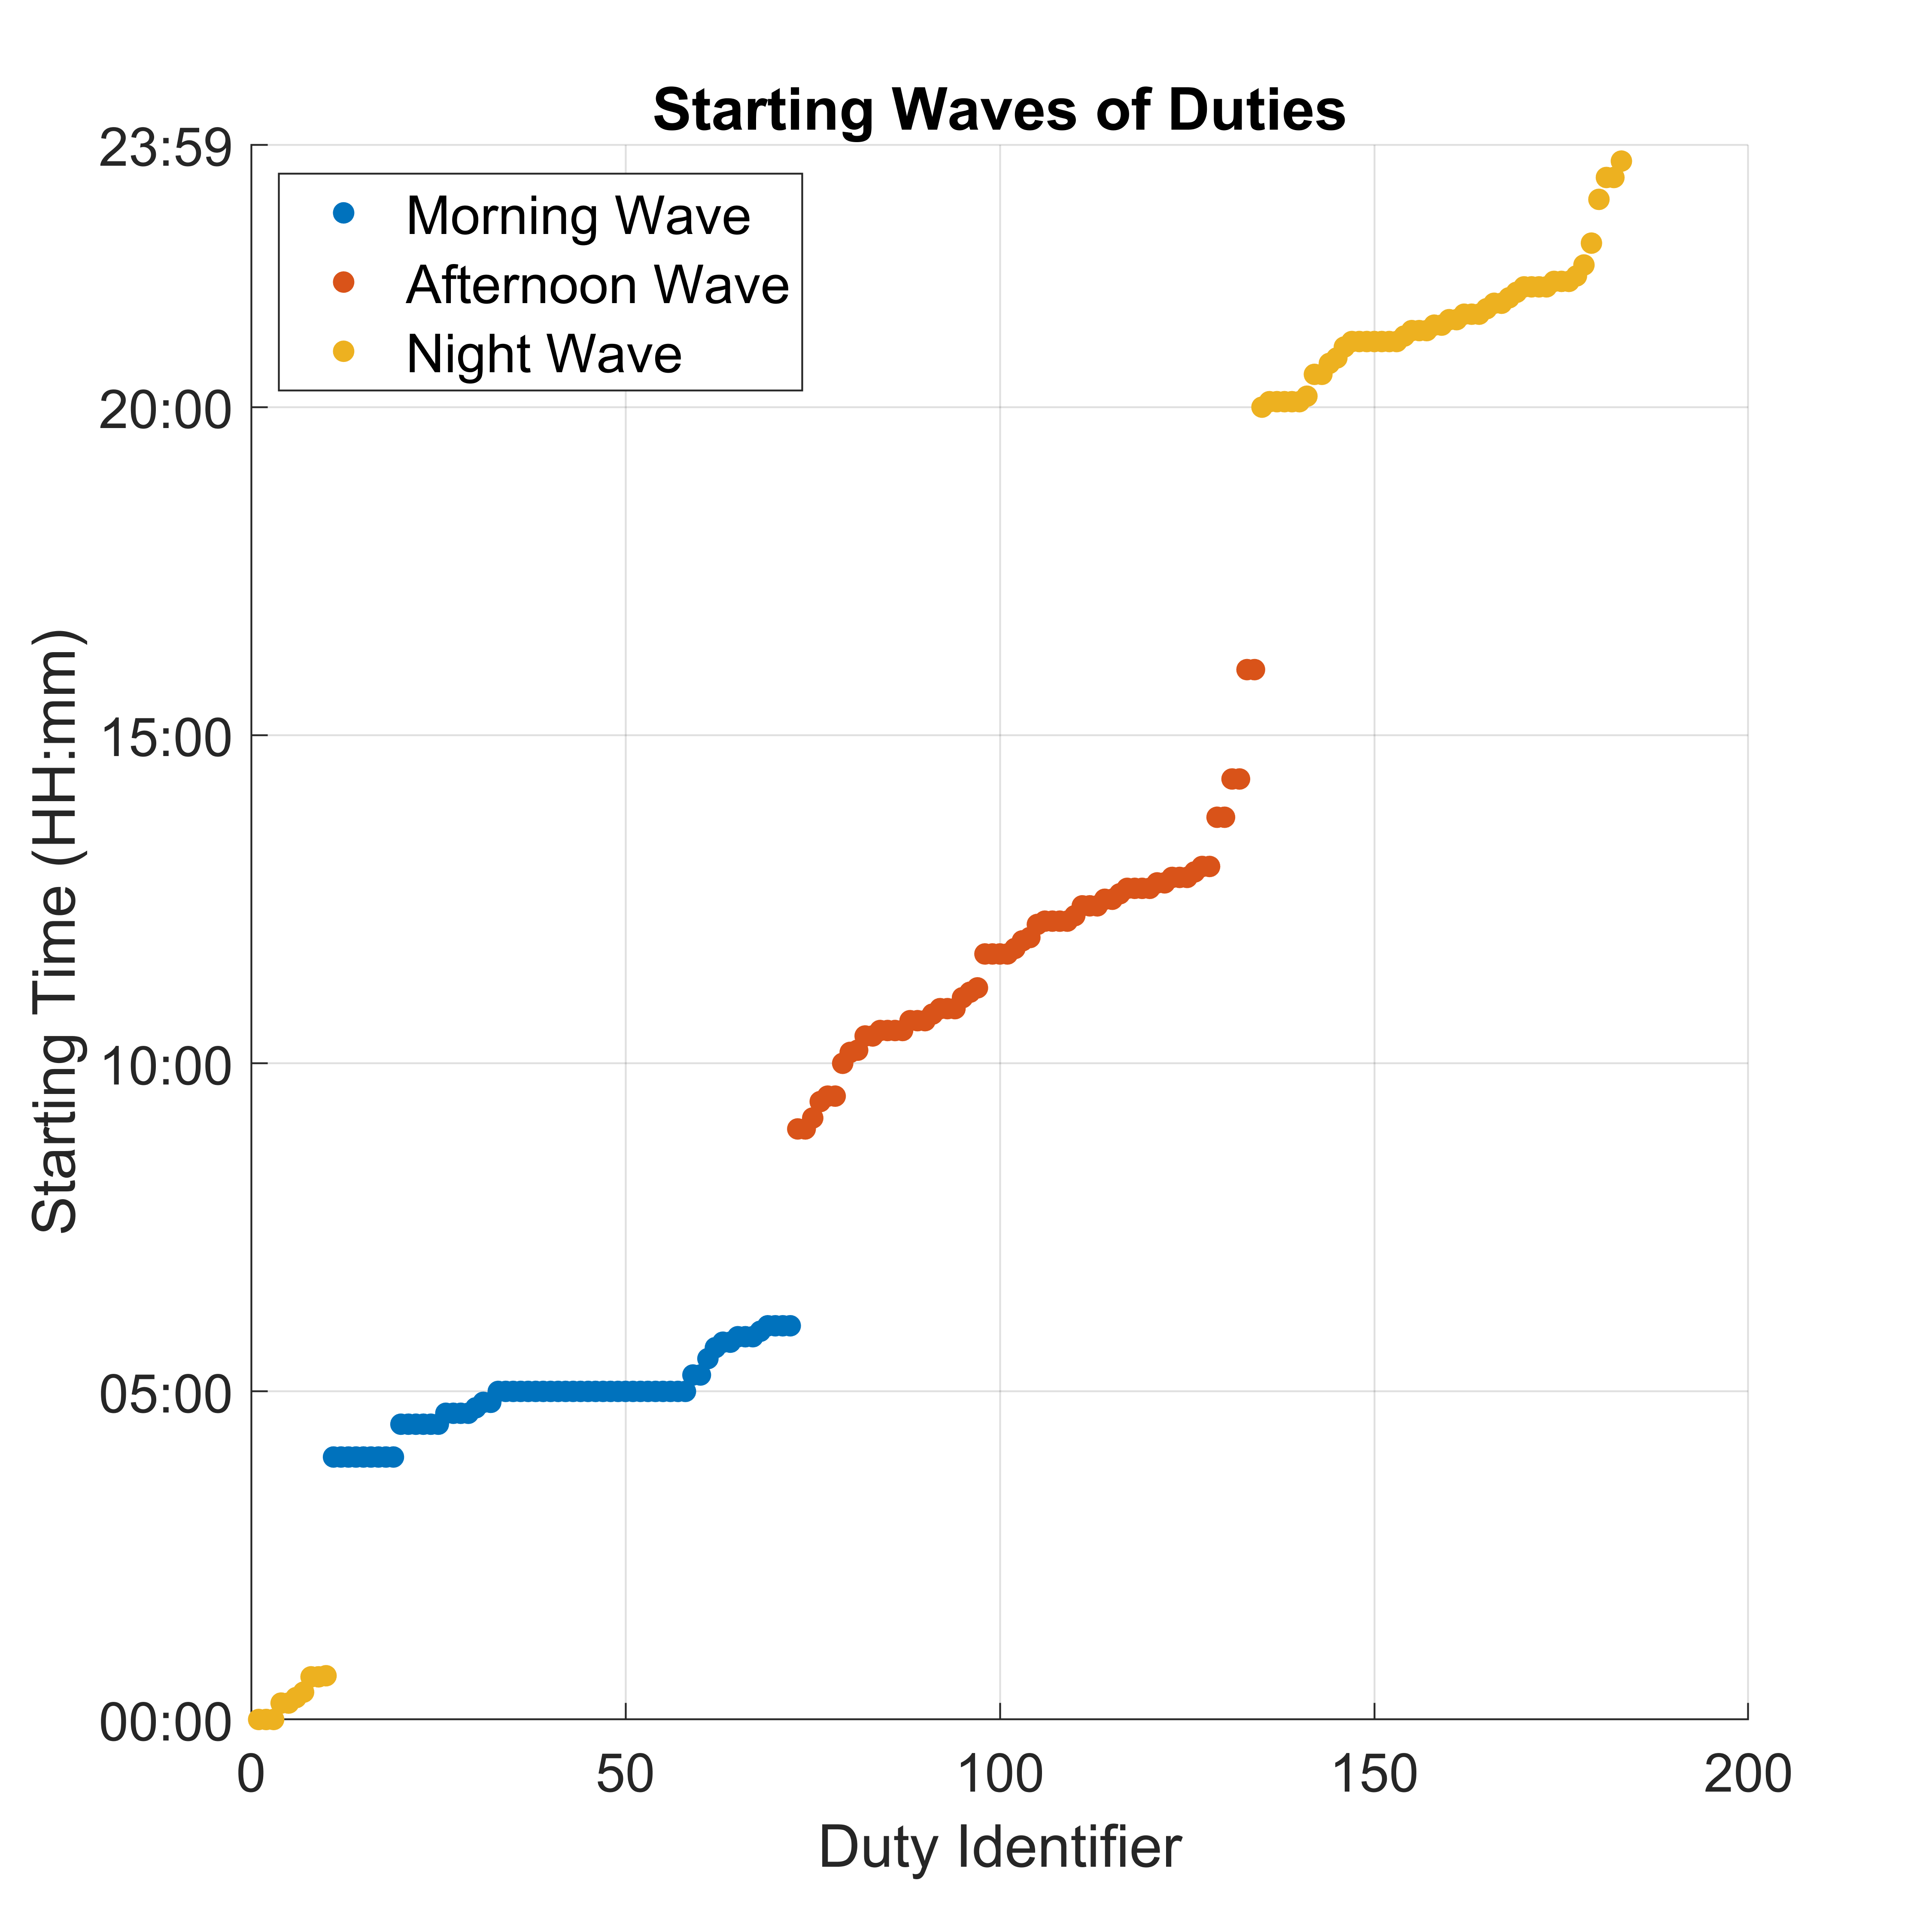
\includegraphics[width=0.46\linewidth]{appendix/Appendix-Start-wave.png}
    
\end{center}
   \caption{Plot of the starting times of duties, illustrating the wave like fashion of the starts of duties.}
\label{fig:starting time}
\end{figure}

\vspace{\baselineskip}
\noindent
Using Figure \ref{fig:starting time} as our guide, we manually characterised each cluster of starting times of duties as \textbf{wave instances}, splitting our overall dataset into the \textbf{three wave sub-instances} of Table \ref{table:Starting Waves} as outlined in Section \ref{section: Wave Instances - Data}.  

%%%%%%%%%%%%%%%%%%%%%%%%%%%%%%%%%%%%%%%%%%%%%%%%%%%%%%% Table %%%%%%%%%%%%%%%%%%%%%%%%%%%%%%%%%%%%%%%%%%%%%%%%%%%%%%%%%%%%%%%%%%%%%%%%%%%

\begin{table}[ht]
\small
    \centering 
    \begin{tabular}{|l|c|c|c|c|}
        \hline
        \textbf{Wave} & \multicolumn{4}{|c|}{ \textbf{Characteristics}} \\
        \hline
        & \textit{Start time} & \textit{End time} & \textit{Timespan}  & \textit{Number of Duties}  \\
        \hline
        \texttt{morning} & 4:00 AM & 6:00 AM & 2 hours & 60 \\
        \hline
        \texttt{afternoon} & 9:00 AM & 4:00 PM & 7 hours & 60 \\
        \hline
        \texttt{night} & 8:00 PM & 0:40 PM & 4 hours, 40 minutes & 63 \\
        \hline
    \end{tabular}%
    \medbreak
    \caption{Table outlining the Starting time, End time and Number of duties of each wave. Time values are stated in (HH:mm) AM/PM units.}
    \label{table:Starting Waves}
\end{table}

\vspace{\baselineskip}
\noindent
As we can see in Table \ref{table:Starting Waves} the waves have practically the same amount of duties, however they differ considerably in their timespan. The \texttt{morning} wave is around half the length of the \texttt{night} wave, and the \texttt{afternoon} is almost equal to the sum of the \texttt{morning, night} waves.    

%%%%%%%%%%%%%%%%%%%%%%%%%%%%%%%%%%%%%%%%%%%%%%%%%%%%%%%% sub-Section %%%%%%%%%%%%%%%%%%%%%%%%%%%%%%%%%%%%%%%%%%%%%%%%%%%%%%%%%%%%%%%%%%%%%%%%%
\subsection{Number of Daily Duties}
We thought, it would be an interesting fact to see how many duties occurred each day of the week. This information was deduced from our dataset which contained one week's worth of duties. We plotted the number of duties that occurred each day on Figure \ref{fig: Number of shifts per day}. The findings from this plot would consequently, be indicative of the number of HGV drivers required to carry out those duties per week. Hence, we can infer what Royal Mail's overall fleet of drivers looks like on a given week, since each driver performs one duty per day. 

\vspace{\baselineskip}
\noindent
We can observe from the figure that Royal Mail, requires on average around 60 drivers to be active each day of the week. Understandably considerably less drivers are required to carry out the weekend shifts since there is not much activity over the weekend.   

%%%%%%%%%%%%%%%%%%%%%%%%%%%%%%%%%%%%%%%%%%%%%%%%%%%%%%%% Figure %%%%%%%%%%%%%%%%%%%%%%%%%%%%%%%%%%%%%%%%%%%%%%%%%%%%%%%%%%%%%%%%%%%%%%%%%


\begin{figure}[ht]
\begin{center}
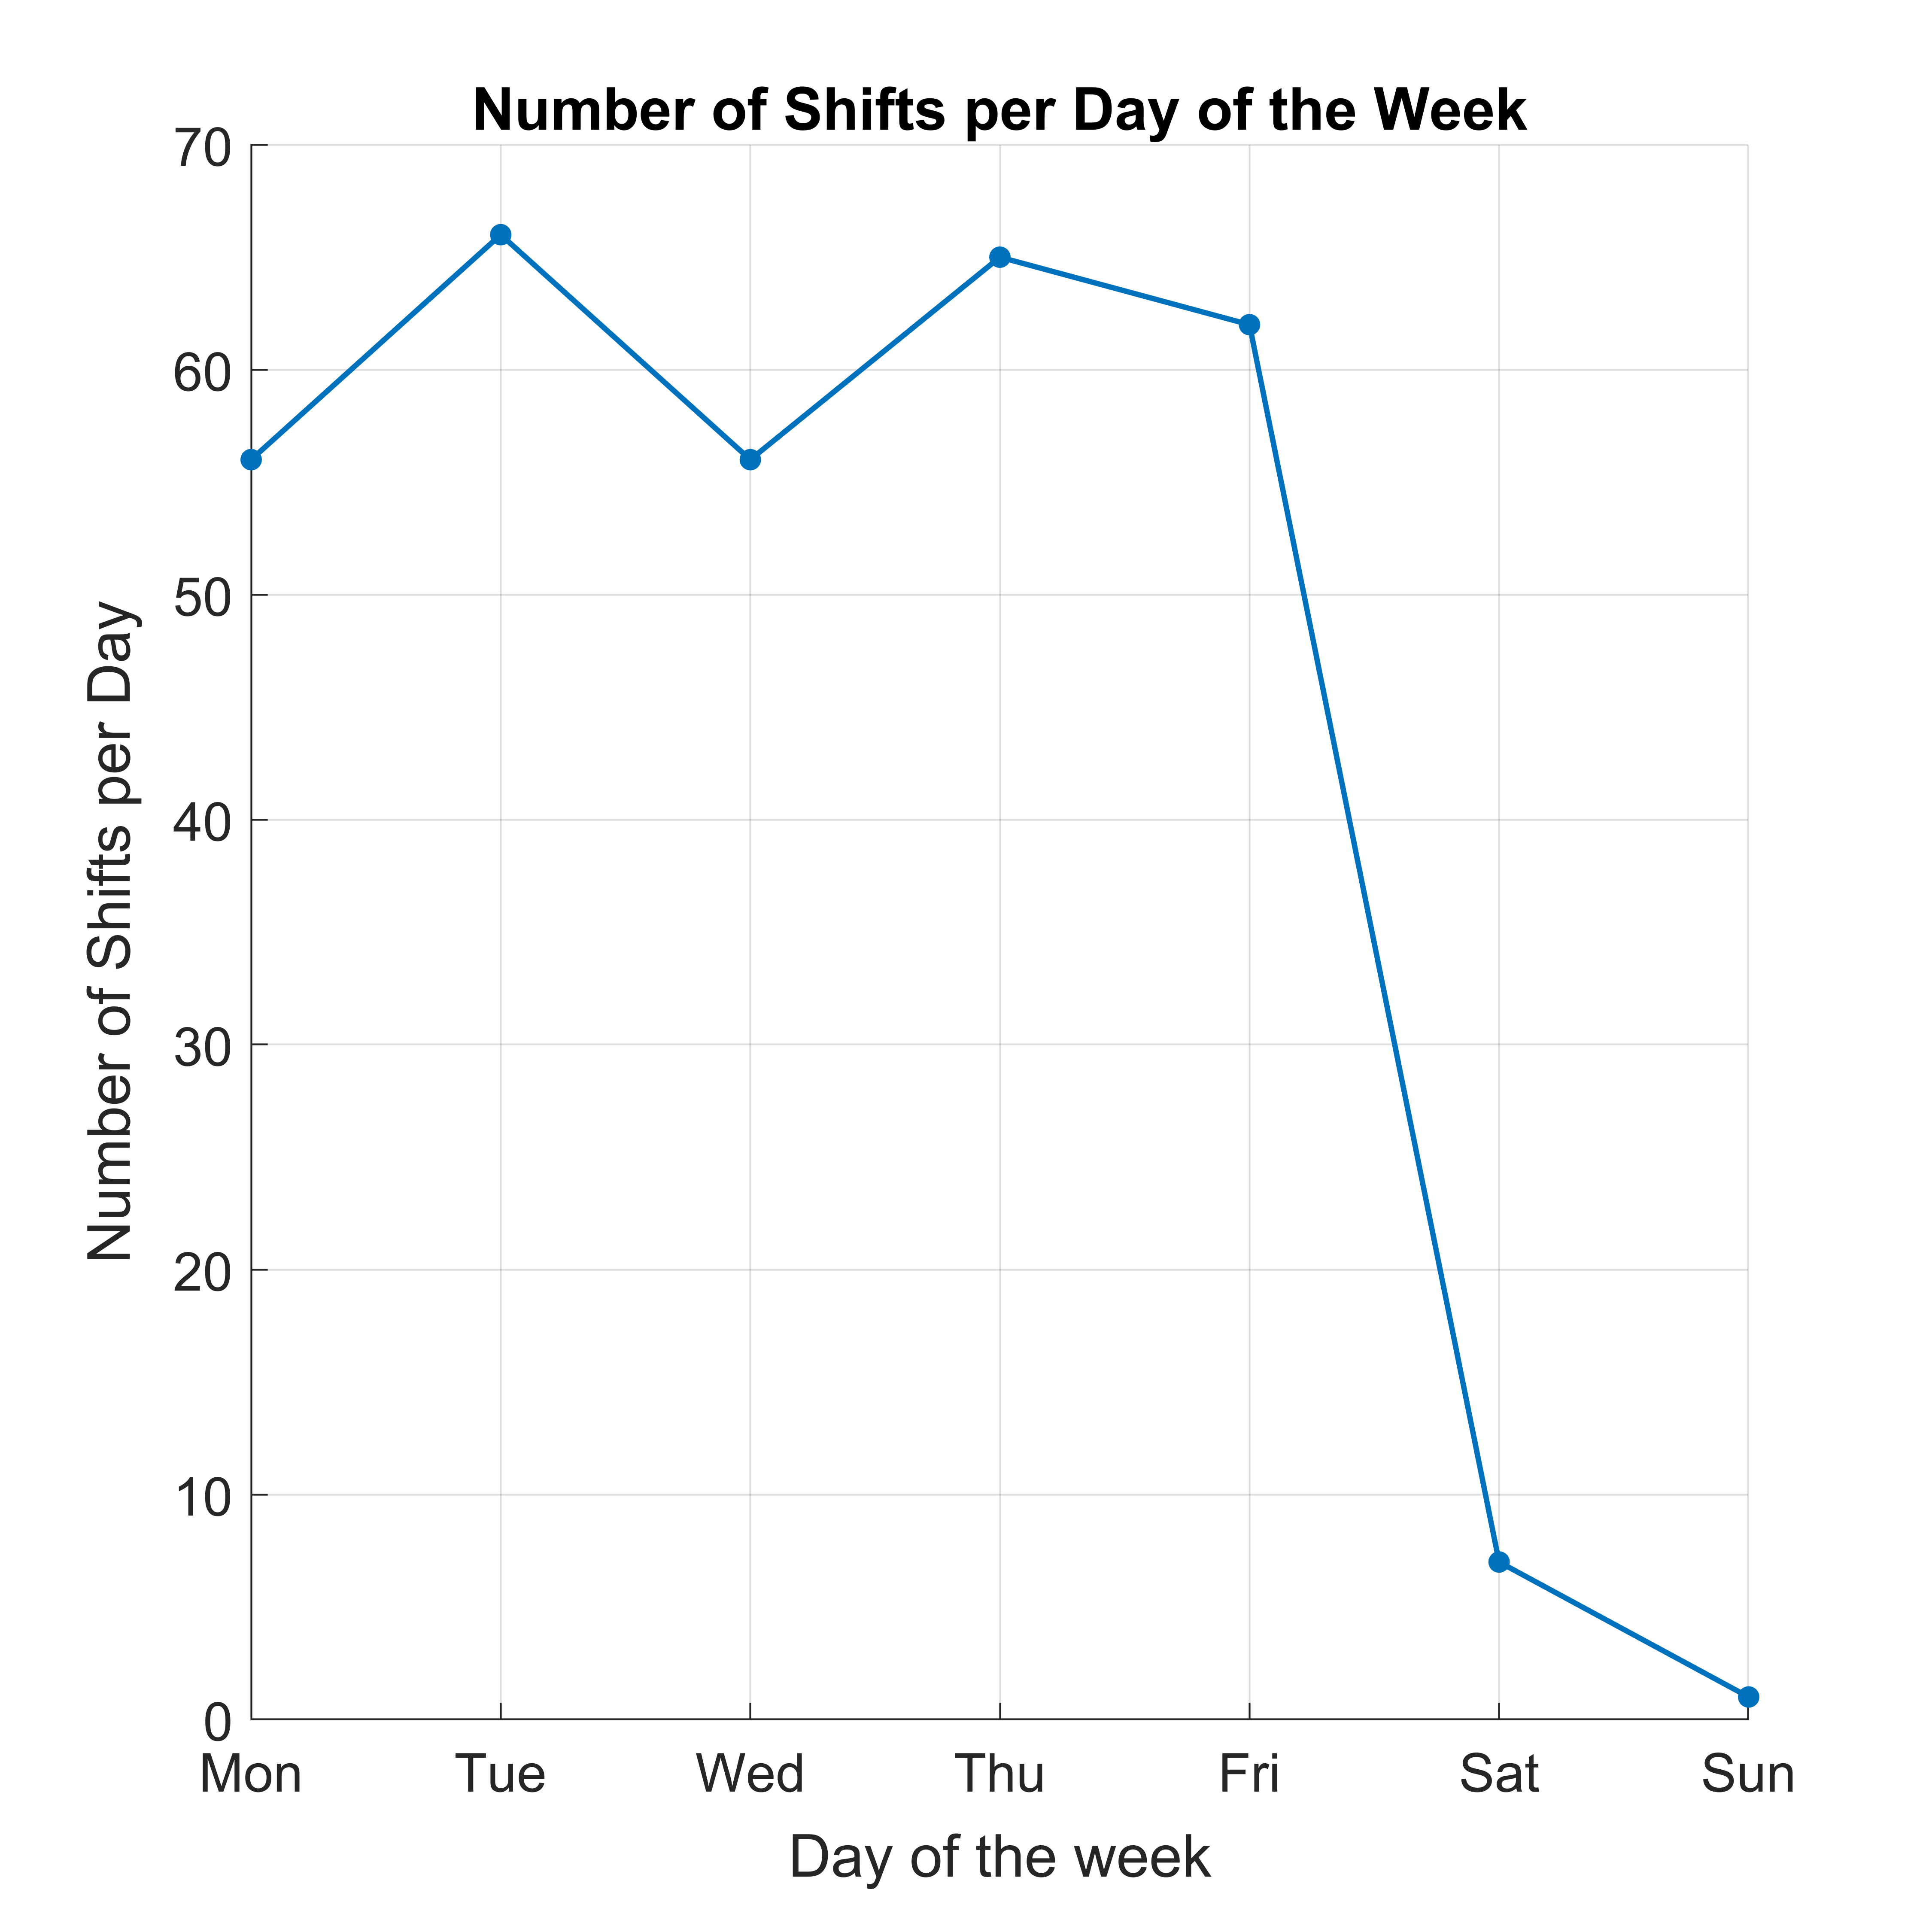
\includegraphics[width=0.46\linewidth]{appendix/shift per day.png}
    
\end{center}
   \caption{Plot of the number of shifts occurring each day.}
\label{fig: Number of shifts per day}
\end{figure}

%%%%%%%%%%%%%%%%%%%%%%%%%%%%%%%%%%%%%%%%%%%%%%%%%%%%%%%% Section %%%%%%%%%%%%%%%%%%%%%%%%%%%%%%%%%%%%%%%%%%%%%%%%%%%%%%%%%%%%%%%%%%%%%%%%%

\section{Operations on Historical Schedules}

%%%%%%%%%%%%%%%%%%%%%%%%%%%%%%%%%%%%%%%%%%%%%%%%%%%%%%%% Sub-Section %%%%%%%%%%%%%%%%%%%%%%%%%%%%%%%%%%%%%%%%%%%%%%%%%%%%%%%%%%%%%%%%%%%%%%%%%
\subsection{Redefining Historical Schedules}
\label{subsection: redefine appexnix}
%%%%%%%%%%%%%%%%%%%%%%%%%%%%%%%%%%%%%%%%%%%%%%%%%%%%%%%%%%%%%%%%%%%%%%%%%%%%%%% Figure %%%%%%%%%%%%%%%%%%%%%%%%%%%%%%%%%%%%%%%%%%%%%%%%%%%%%%%%%%%%%%%%%%%%%%%%%%%%%%

\begin{figure}[ht]
    \centering
    \subfloat[\textit{Duty lengths} sorted in increasing order, showing the effect of deleting the \textbf{non-useful} activities.]{%\begin{center}
    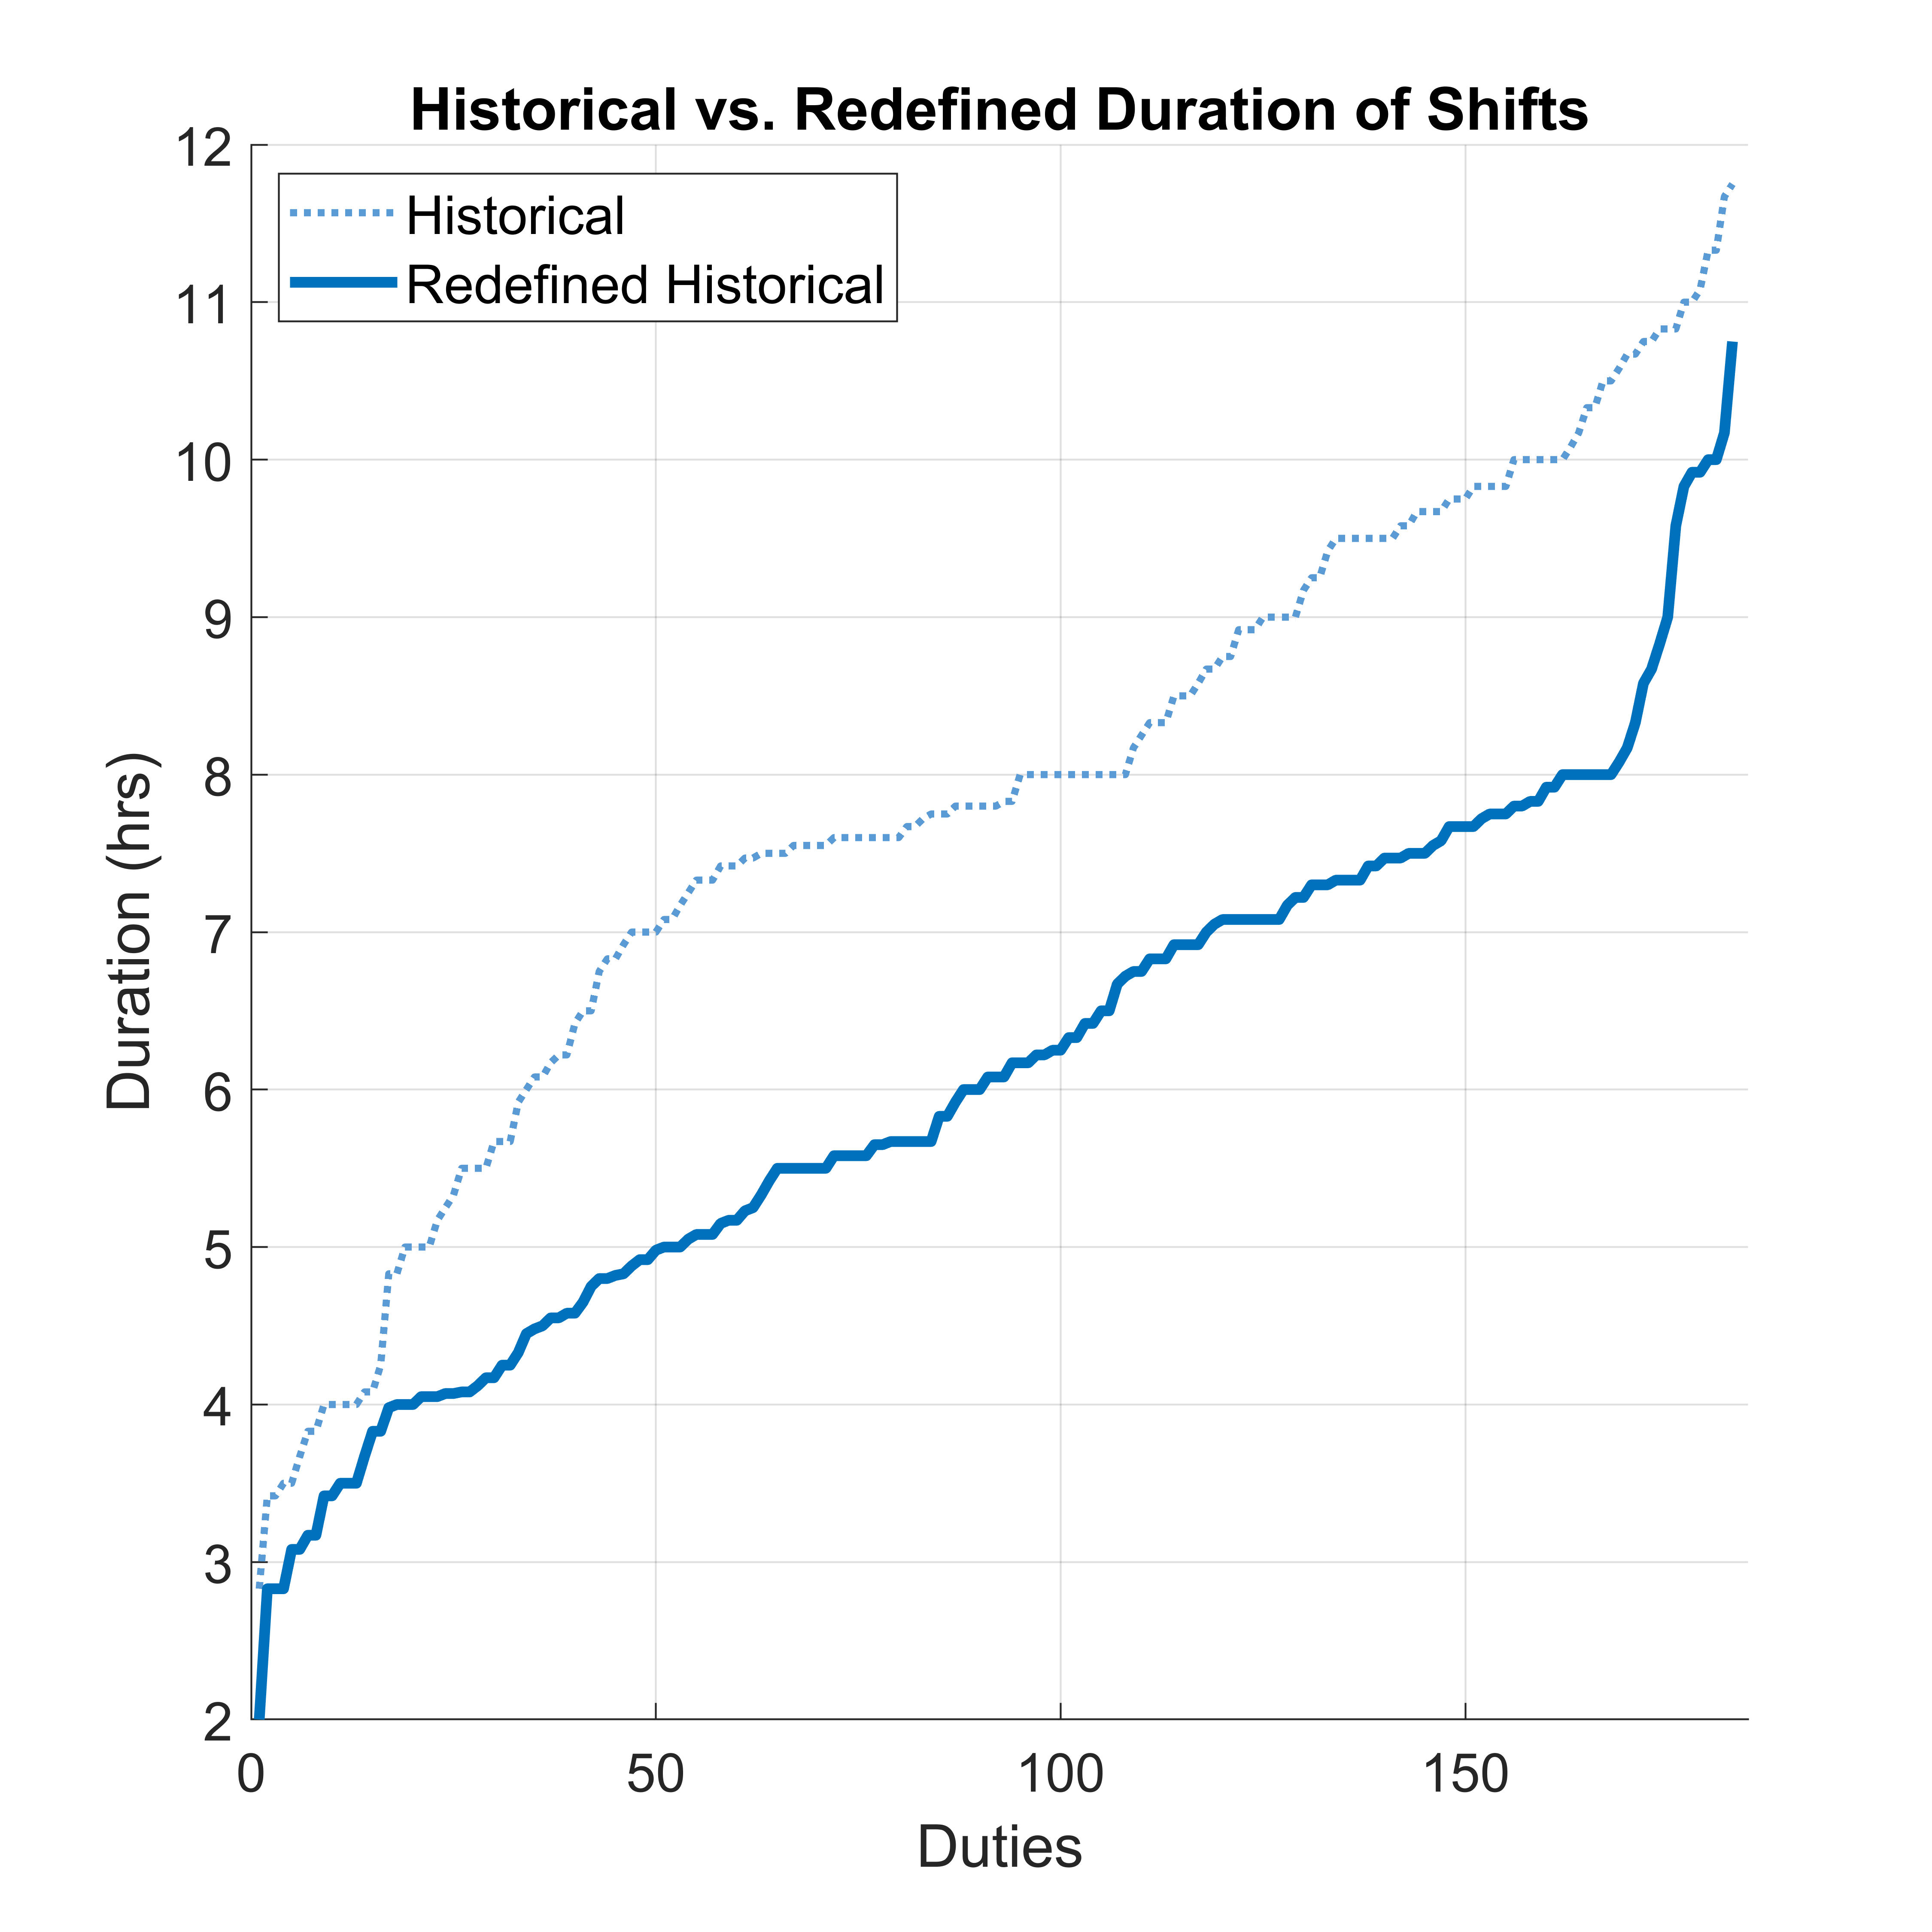
\includegraphics[width=0.46\linewidth]{[1] - chapter/Image Files/1-Effect-of-Redefined.png}
    }%\end{center}}%picture #1
    \qquad
    %picture #2
    \centering
    \subfloat[Histogram showing the effect of Redefining the dataset.]{%\begin{center}
    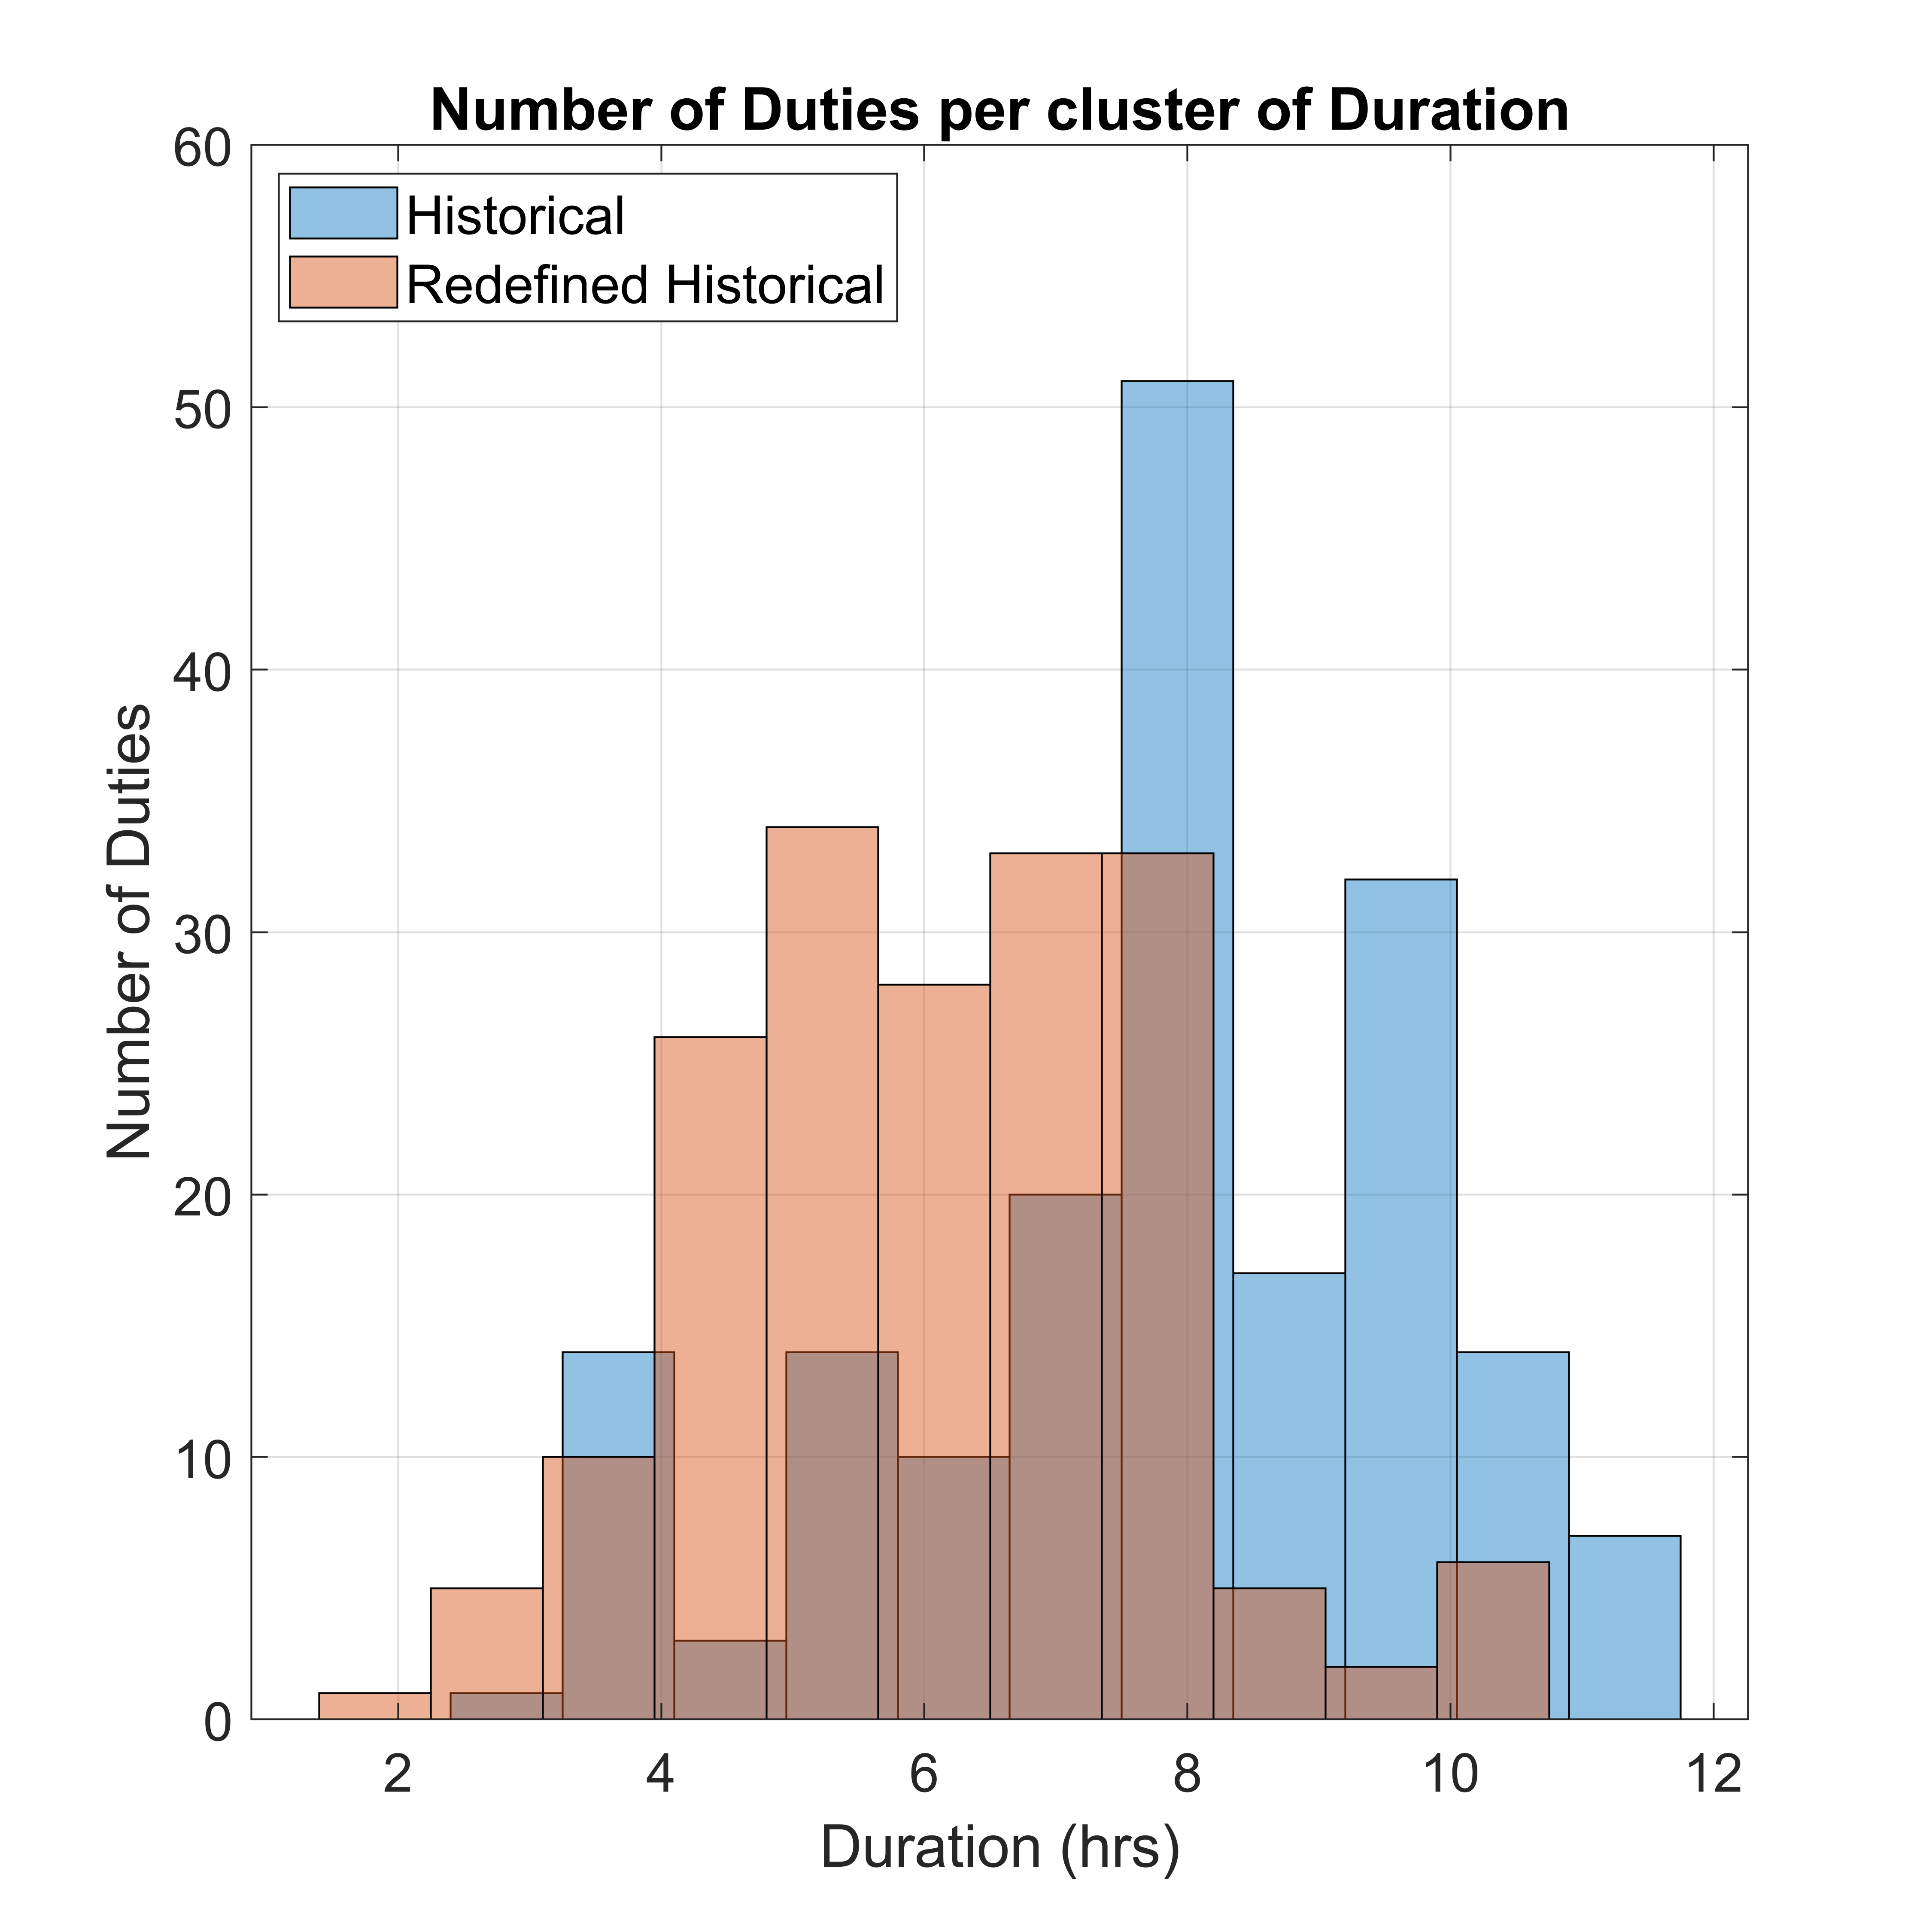
\includegraphics[width=0.46\linewidth]{[1] - chapter/Image Files/1-Effect-of-Redefined-histogram.png}
    }%\end{center}}%end of picture #2
    \caption{Figures illustrating the effects of the Redefining the dataset by deleting the \textbf{non-useful} activities from the Historical Schedule.}%
    \label{fig: Redefined Historical.}%
\end{figure}

In this section we discuss the effects of the operation carried out in Section \ref{section: Redefined Dataset} regarding the deletion of \textbf{non-useful} activities from the original dataset. As one can see Figure \ref{fig: Redefined Historical.}(a) there is a step change deletion of overall time to be schedule from the Historical dataset, once we delete the non-useful activities. Subsequently, Figure \ref{fig: Redefined Historical.}(b) shows the same effect as observed in a histogram graph. The deletion of the non-useful time is observed as a horizontal shift to of the histogram to the left, signifying the fact that less overall hours are not contained in the schedule.

\vspace{\baselineskip}
\noindent
The operation of deleting the activities has a direct impact on the structure of the blocks. Namely, blocks that contain such \textbf{non-useful} activities will see their duration decreased. This is seen more practically in the following table:

%%%%%%%%%%%%%%%%%%%%%%%%%%%%%%%%%%%%%%%%%%%%%%%%%%%%%%%%%%%%%%%%%%%%%% Table %%%%%%%%%%%%%%%%%%%%%%%%%%%%%%%%%%%%%%%%%%%%%%%

\begin{table}[ht]
\small
    \centering 
    \begin{tabular}{|c|c|c|c|}
        \hline
        \textbf{Instance} & \multicolumn{3}{|c|}{ \textbf{Blocks (HH:mm)}}  \\
        \hline
         & \texttt{Average} &  \texttt{Minimum} & \texttt{Maximum} \\
        \hline
        Historical & 03:05 & 00:40 & 08:25 \\
        \hline
        Morning & 03:28 & 00:50 & 08:25 \\
        \hline
        Afternoon & 03:05 & 01:10 & 07:20 \\
        \hline
        Night & 02:52 & 00:40 & 07:30 \\
        \hline
    \end{tabular}%
    \medbreak
\end{table}

%%%%%%%%%%%%%%%%%%%%%%%%%%%%%%%%%%%%%%%%%%%%%%%%%%%%%%%% Sub-Section %%%%%%%%%%%%%%%%%%%%%%%%%%%%%%%%%%%%%%%%%%%%%%%%%%%%%%%%%%%%%%%%%%%%%%%%%

\subsection{Comparison of Disturbed Nominal and Optimised Schedules}
\label{subsection: Appendix Comparison of Disturbed Nominal and Optimised Schedules}
In Figure \ref{fig: Nominal Uncertainty Sets Effects.} our goal is to determine the robustness to uncertainty of the nominal schedule. To identify its level of robustness we compare, for of the three uncertainty sets, the disturbed instance optimised under uncertainty with the nominal schedule disturbed with the same instance. There are two such cases for each uncertainty set, one that involves instances that have been \texttt{reduced}, with respect to the overall time scheduled, after the application of uncertainty, and those that have been \texttt{augmented} respectively. The former are presented in Figure \ref{fig: Nominal Uncertainty Sets Effects.}(a) while the latter in Figure \ref{fig: Nominal Uncertainty Sets Effects.}(b). 

%%%%%%%%%%%%%%%%%%%%%%%%%%%%%%%%%%%%%%%%%%%%%%%%%%%%%%% Double Figure %%%%%%%%%%%%%%%%%%%%%%%%%%%%%%%%%%%%%%%%%%%%%%%%%%%%%%%%%%%%%%%%%%%%%%%%%%%

\begin{figure}[ht]
    \centering
    \subfloat[Disturbed instances with a \textbf{decrease} in overall labor time (\texttt{reduced}).]{%\begin{center}
    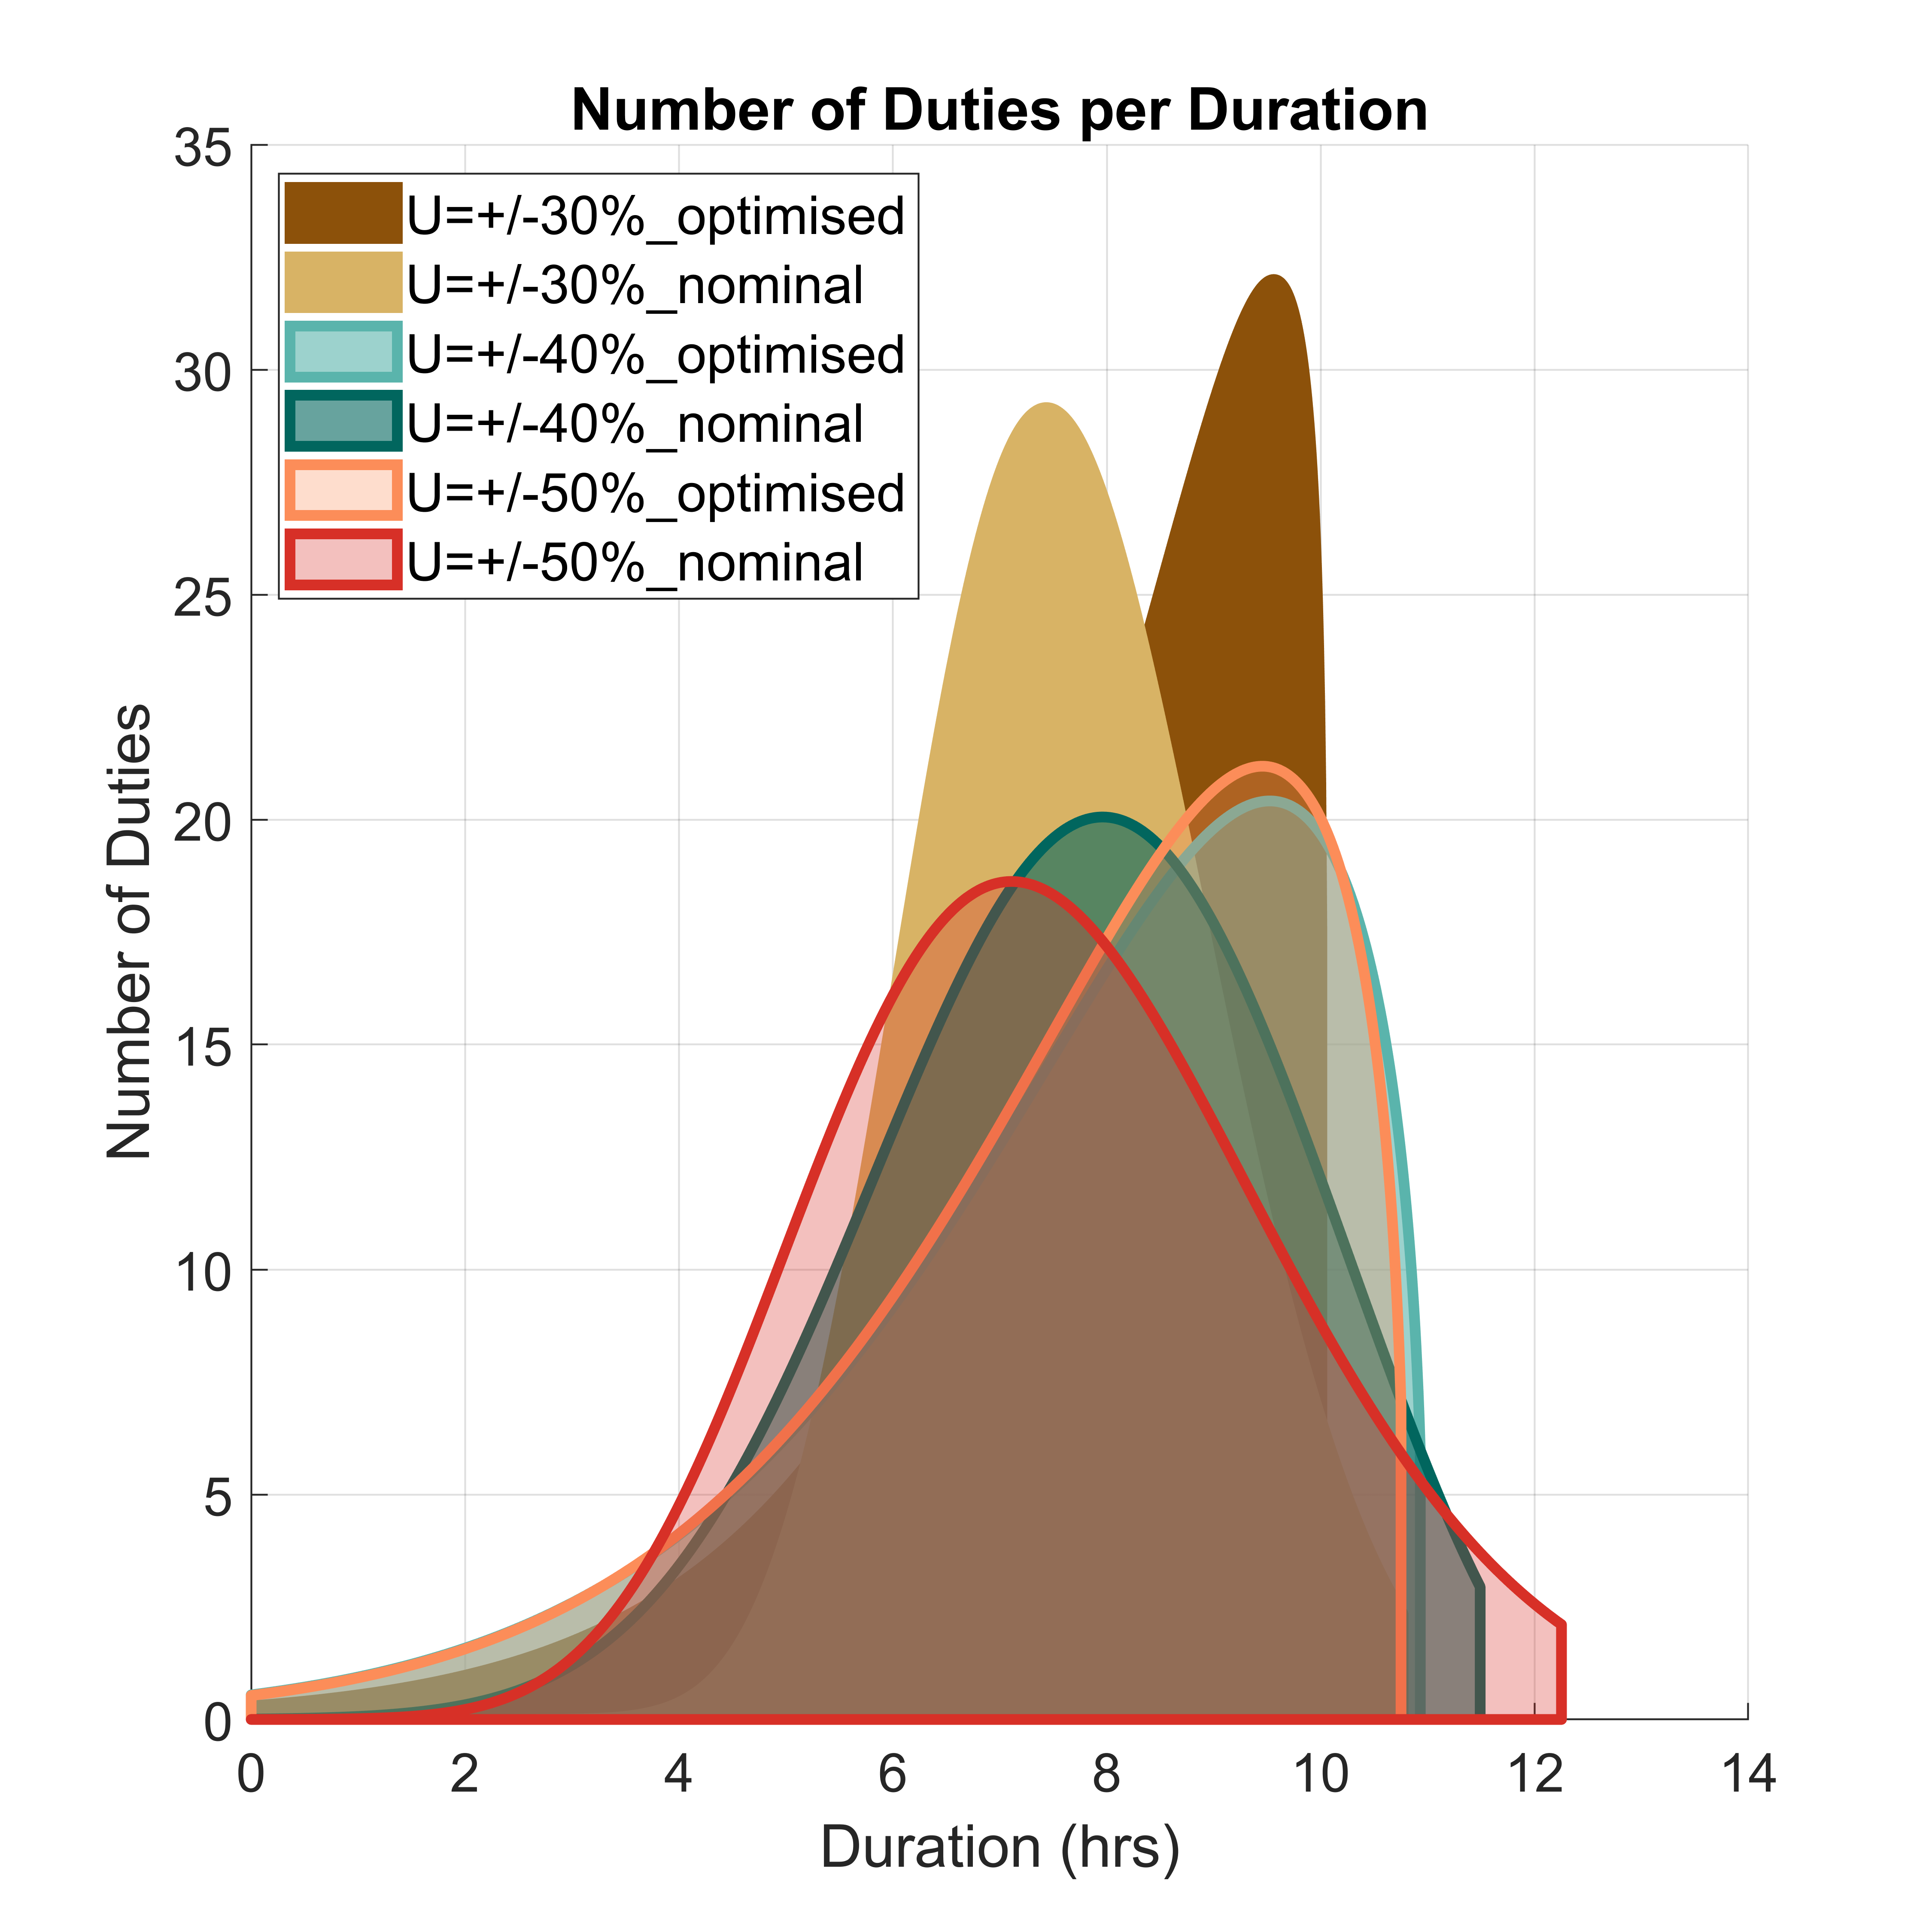
\includegraphics[width=0.46\linewidth]{appendix/Comparison_Of_Uncertainty_Sets_min_and_nominal.png}
    }%\end{center}}%end of picture #2
    \qquad
    %picture #2
    \centering
    \subfloat[Disturbed instances with an \textbf{increase} in overall labor time (\texttt{augmented}).]{%\begin{center}
    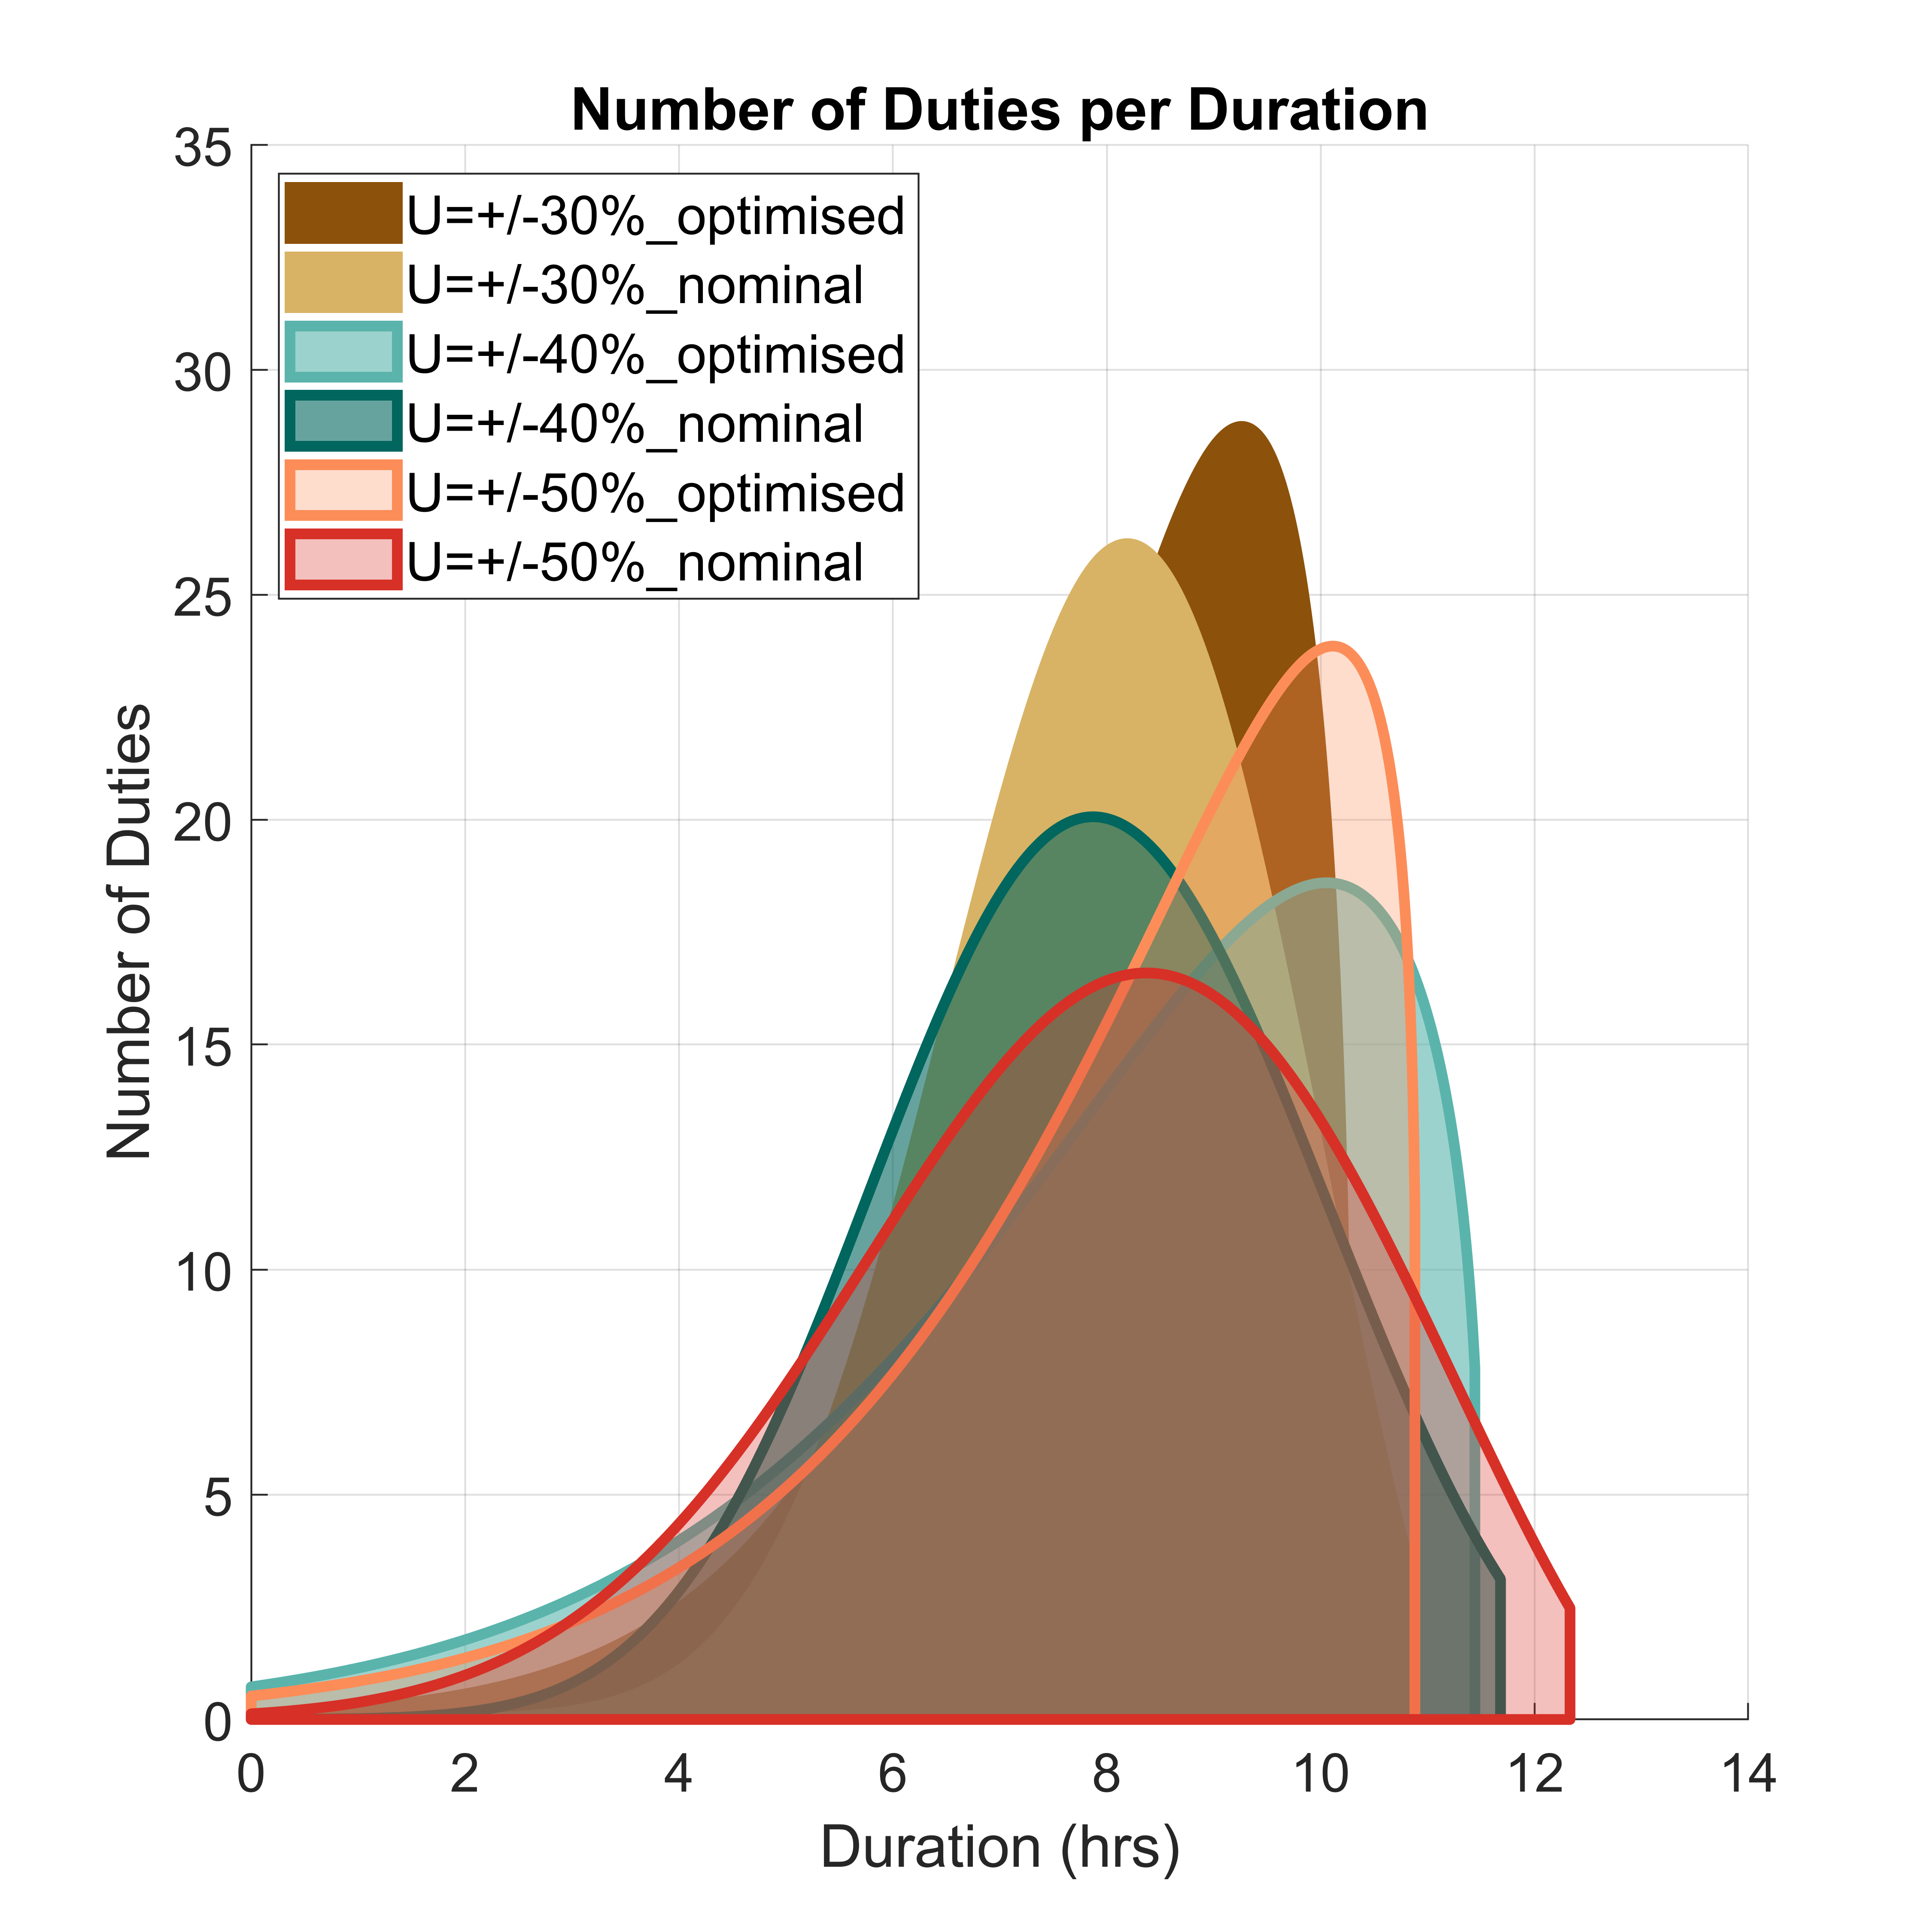
\includegraphics[width=0.46\linewidth]{appendix/Comparison_Of_Uncertainty_Sets_max_and_nominal.png}
    }%\end{center}}%picture #1
    \caption{The histograms provide an overview of the effects of various levels of uncertainty set on $Duty$ lengths.}
    \label{fig: Nominal Uncertainty Sets Effects.}
\end{figure}
 



%%%%%%%%%%%%%%%%%%%%%%%%%%%%%%%%%%%%%%%%%%%%%%%%%%%%%%%% Section %%%%%%%%%%%%%%%%%%%%%%%%%%%%%%%%%%%%%%%%%%%%%%%%%%%%%%%%%%%%%%%%%%%%%%%%%
\section{Supporting Notes}

%%%%%%%%%%%%%%%%%%%%%%%%%%%%%%%%%%%%%%%%%%%%%%%%%%%%%%%% Sub-Section %%%%%%%%%%%%%%%%%%%%%%%%%%%%%%%%%%%%%%%%%%%%%%%%%%%%%%%%%%%%%%%%%%%%%%%%%

\subsection{EU Directives for HGV Drivers}
\label{section: EU rules}
This section makes reference to the  European Union (EU) rules on drivers' hours and working time as dictated by the Department for Transport (DfT). This is an important real-life aspect of our problem, that is mentioned and referred to, at various points in the report. %link: https://assets.publishing.service.gov.uk/government/uploads/system/uploads/attachment_data/file/856360/simplified-guidance-eu-drivers-hours-working-time-rules.pdf

\begin{enumerate}[label=\textbf{(\arabic*)}]
    \item \textbf{\underline{Driving-time Directive}: }
       
       \vspace{\baselineskip}
        \noindent
        \begin{enumerate}[label=\roman*]
       \item \underline{Time Limit:}
       
        \begin{itemize}
            \item 9 hours daily driving limit.
            \item Maximum of 56 hours weekly driving limit.      
            \item Maximum of 90 hours fortnightly driving limit.
        \end{itemize} 
        
        \vspace{\baselineskip}
        \noindent
      \item  \underline{Break:}
        \begin{itemize}
        \item 45 minutes break after 4.5 hours driving
        \end{itemize} 
        \end{enumerate}

    \item \textbf{\underline{Working-time Directive}: }
    
      \vspace{\baselineskip}
      \noindent
      \begin{enumerate}[label=\roman*]
    \item  \underline{Time Limit:}
    
        \begin{itemize}
            \item Working time must not exceed average of 48 hours a week.
            \item Maximum working time of 60 hours in one week.
            \item Maximum working time of 10 hours if night work performed.
        \end{itemize}  
        
        
        \vspace{\baselineskip}
        \noindent
    \item    \underline{Break:}
        \begin{itemize}
        \item Cannot work for more than 6 hours without a break. A break should be at least 15 minutes long
        \item 30 minute break if working between 6 and 9 hours in total
        \item 45 minute break if working more than 9 hours in total
        \end{itemize} 
        \end{enumerate}

\end{enumerate}

        
%%%%%%%%%%%%%%%%%%%%%%%%%%%%%%%%%%%%%%%%%%%%%%%%%%%%%%%% Sub-Section %%%%%%%%%%%%%%%%%%%%%%%%%%%%%%%%%%%%%%%%%%%%%%%%%%%%%%%%%%%%%%%%%%%%%%%%%        
\subsection{Relaxation of a Mathematical Program}
\label{section: Appednix Relaxation}
In order to utilise the efficacy of the simplex algorithm, and apply to solve MILPs we require to obtain the relaxation of an integer-linear program into a LP. A relaxed version of an integer program is defined as below.

\begin{equation}
\begin{aligned}
& \underset{x}{\text{minimise}}
& & f(x) \\
& \text{subject to}
& & h_i(x) = 0 \\
& & & g_j(x) \leq 0 \\
\end{aligned}
\end{equation}
\[\text{where} \; x \in S_{original}\]

\noindent
with the corresponding \textbf{relaxed} version of the problem,\par

\begin{equation}
\begin{aligned}
& \underset{x}{\text{minimise}}
& & f(x) \\
& \text{subject to}
& & h_i(x) = 0 \\
& & & g_j(x) \leq 0 \\
\end{aligned}
\end{equation}
\[\text{where} \; x \in S_{relaxed} \; \text{and} \; S_{original} \subseteq S_{relaxed}\]

\vspace{\baselineskip}
\noindent
The relaxation of a problem is usually obtained by the removal of one or more constraints of the original formulation. For example, when obtaining the relaxation of an integer program, we usually refer to the process of neglecting the integrality constraint on the integer program's decision variable(s) to transform our problem into a standard LP.




